Virtuální realita (často zkracována na VR) je bezesporu novým trendem v
oblasti informačních technologií. Protože je tato technologie běžným
lidem méně dostupná, vznikly ve větších městech nové podniky, které
zprostředkovávají zážitky ve virtuální realitě za zlomek ceny celého
systému bez nutnosti znalosti systémů virtuální reality, zajištění
dostatečného výpočetního výkonu, výběru a nákupu aplikací pro virtuální
realitu kompatibilní s konkrétním systémem a konfigurace virtuální
reality. Tyto podniky se označují jako \emph{herny virtuální reality}. \autocite{herny}

Návštěvníci pak kladou na takové podniky jisté požadavky, na které
systémy virtuální reality nejsou v současné době plně připraveny.
Uživatelské rozhraní softwaru je navrženo spíše na jednoho dlouhodobého
uživatele, který měl prostor systému porozumět, což je nevhodné v
prostředí, kde se uživatel s virtuální realitou setkává poprvé a v
omezeném čase, po který mu byl systém zapůjčen.

\section{Co je virtuální
realita}\label{co-je-virtuuxe1lnuxed-realita}

Pojem virtuální realita označuje technologii prezentace prostředí pomocí
replikace lidských smyslů tak, aby simulovala přítomnost uživatele v
takovém prostředí. Často se virtuální realitou označuje i samotné
prostředí. Technologie tak vytváří iluzi reálného alternativního světa. \autocite{ovr}

Konkrétní definici virtuální reality v angličtině: ``a realistic and
immersive simulation of a three-dimensional 360-degree environment,
created using interactive software and hardware, and experienced or
controlled by movement of the body'' \autocite{vrdef} lze přeložit jako ``realistická a
pohlcující simulace trojrozměrného 360 stupňového prostředí tvořeného
pomocí interaktivního softwaru a hardwaru ovládaného pohybem lidského
těla''.

Uživatel virtuální reality se může v prostředí typicky rozhlížet,
procházet se (v různě omezené míře) a interagovat s vyzobrazenými
objekty. \autocite{vrdef2} Virtuální realita nalézá uplatnění v průmyslu, lékařství,
sportu, armádě a především i v zábavním průmyslu. \autocite{vrusage}

Počátky virtuální reality sahají až do 50. let 18. století, kdy se
experimentovalo s různými stereoskopickými displeji a zprostředkováním
jevů ostatních lidských smyslů. Jako nejranější známý příklad virtuální
reality je přístroj zvaný \emph{Sensorama}, který byl schopen zobrazovat
trojrozměrné stereoskopické obrázky, přehrávat zvuk prostředí a
vypouštět aromatické látky pro pohlcující zážitek. \autocite{oldvr}

Na počátku 20. století se objevily další příklady pohlcujících zážitků
virtuální reality. Za zmínku stojí projekční místnost \emph{The Cave},
mezi koncové uživatele nikdy nerozšířený \emph{Sega VR Headset}, či
stejně nepříliš úspěšný \emph{Virtual Boy} od společnosti
\emph{Nintendo}.

\begin{figure}[h!]
\centering
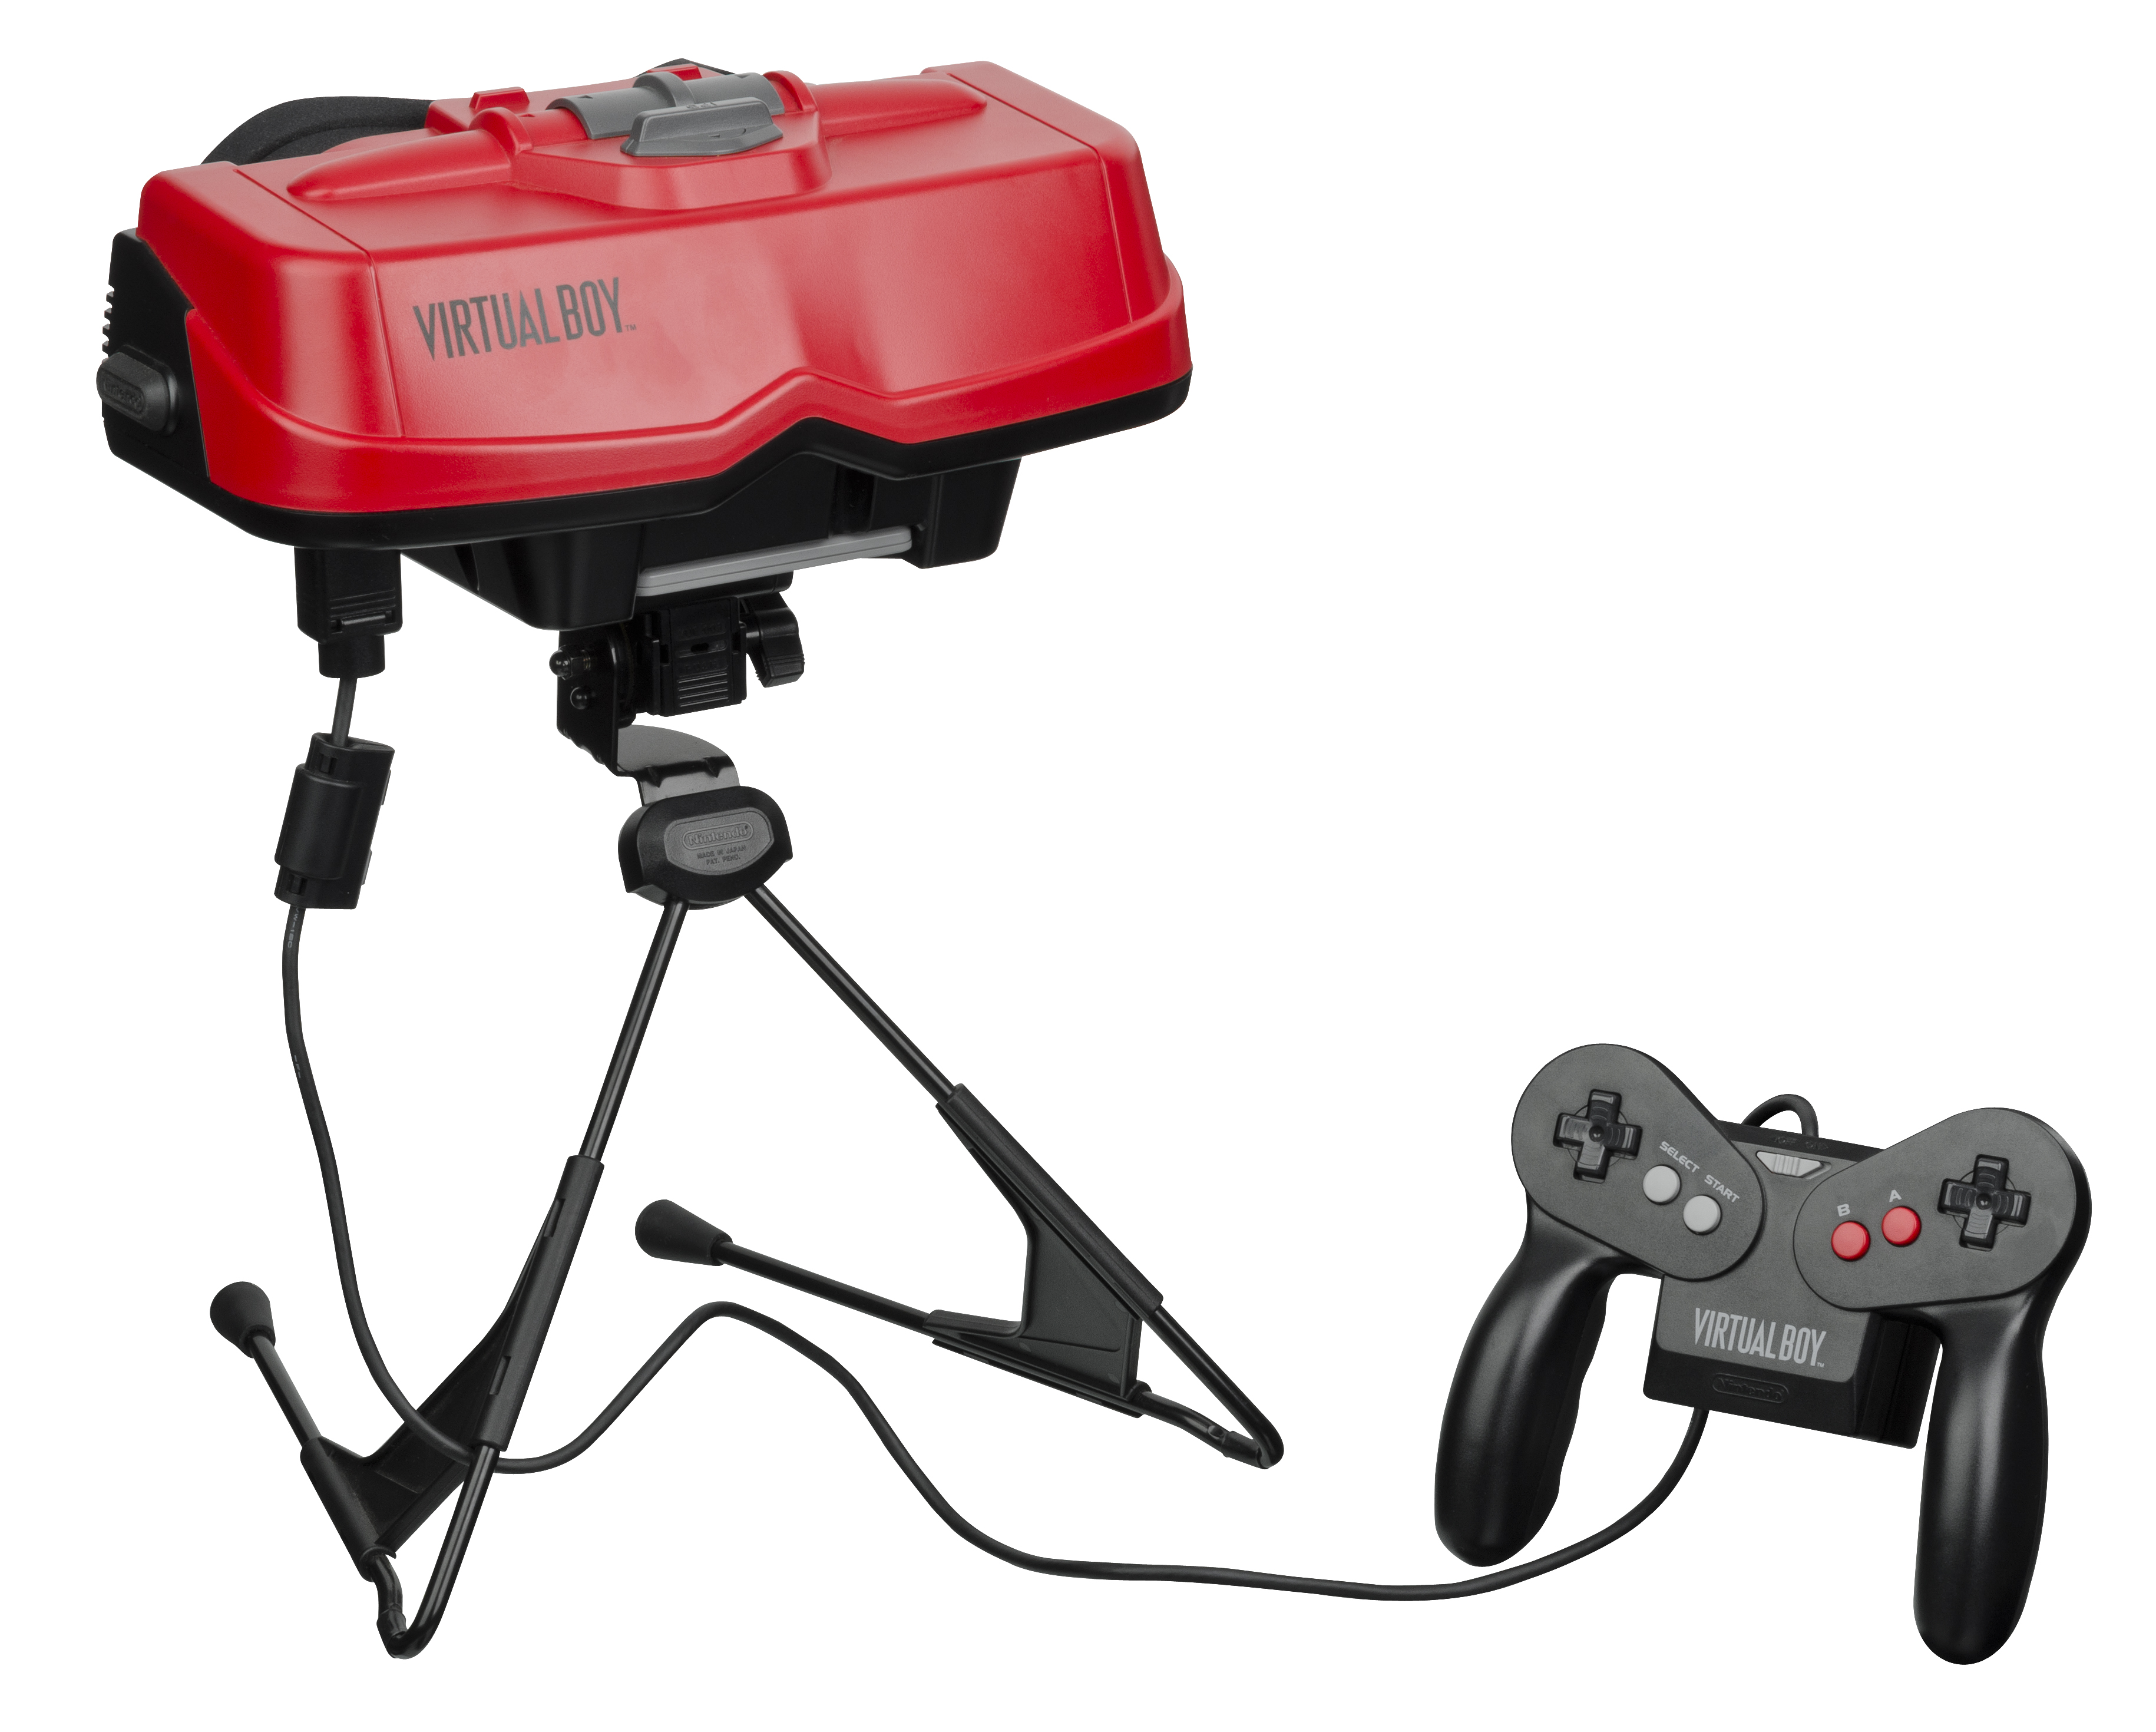
\includegraphics[width=8cm]{src/assets/virtual-boy.jpg}
\caption{Virtuální realita z roku 1995 -- Virtual Boy\autocite{virtualboypic}}
\end{figure}

\section{Virtuální realita v
současnosti}\label{virtuuxe1lnuxed-realita-v-souux10dasnosti}

V současnosti je virtuální realita tvořena typicky pomocí počítačem
generované trojrozměrné grafiky a zvuku, snímání pohybu a snímání polohy
lidského těla. Uživateli je zážitek zprostředkován pomocí náhlavní
soupravy, které vykreslují obraz, přenášejí zvuk a snímají polohu hlavy
uživatele. \autocite{vrnow}

V rámci této technologie tak vznikají celé systémy virtuální reality,
které disponují různými vlastnotmi, různými technologiemi simulace a
různou kvalitou simulace. Některé systémy míru a kvalitu simulace
doplňují snímáním celého lidského těla, či částí jejich končetin, např.
ovladačů pro ruce. Snímány mohou být i polohy fyzických předmětů, či
různých jiných ovladačů. 

Systémy se mohou lišit i technologií snímání.
Některé používají infračervené světlo a kamery, jiné zase laserové
snímání. Virtuální realita pro některá mobilní zařízení například
využívá pouze gyroskopických senzorů.

Velkou roli v této technologii hraje, mimo kvalitní a rychlé gyroskopy,
také počítačový výkon. \autocite{vrtech} Právě kvůli virtuální realitě začal v poslední
době převažovat trend nových ``VR ready'' grafických karet, které jsou
přizpůsobeny k výpočtu obrazu z dvou úhlů pro efekt stereoskopie.

\section{Systém HTC Vive}\label{systuxe9m-htc-vive}

Systém \emph{Vive} vyvinutý společností \emph{HTC} je jedním z
nejoblíbenějších systémů virtuální reality v současnosti. \autocite{vivepopular} Současně s
\emph{HTC} se na vývoji podílela společnost \emph{Valve}. Tato
společnost stojí za jednou z největších platforem pro digitální
distribuci počítačových her -- \emph{Steam}. S touto službou je úzce
spjatá technologie \emph{SteamVR}. O těchto technologiích více
pojednávají kapitoly níže.

Systém \emph{HTC Vive} se skládá z náhlavní soupravy s OLED displejem o
rozlišení 2160x1200 a dvou ovladačů do ruky s gyroskopickými senzory,
senzory detekce pozice v prostoru, pěti tlačítky, dotykovou plochou a
haptickou odezvou. \autocite{vivespec} Díky laserovému snímání je možné velmi přesně snímat
relativně velký prostor v místnosti, ve které se může uživatel volně
pohybovat. V České republice je k současnému datu systém dostupný za
přibližně 24 tisíc korun. \autocite{viveprice} Koncovým zákazníkům se stal dostupným v dubnu
roku 2016. Pro tento systém bude navržena aplikace této závěrečné práce.

\begin{figure}[h!]
\centering
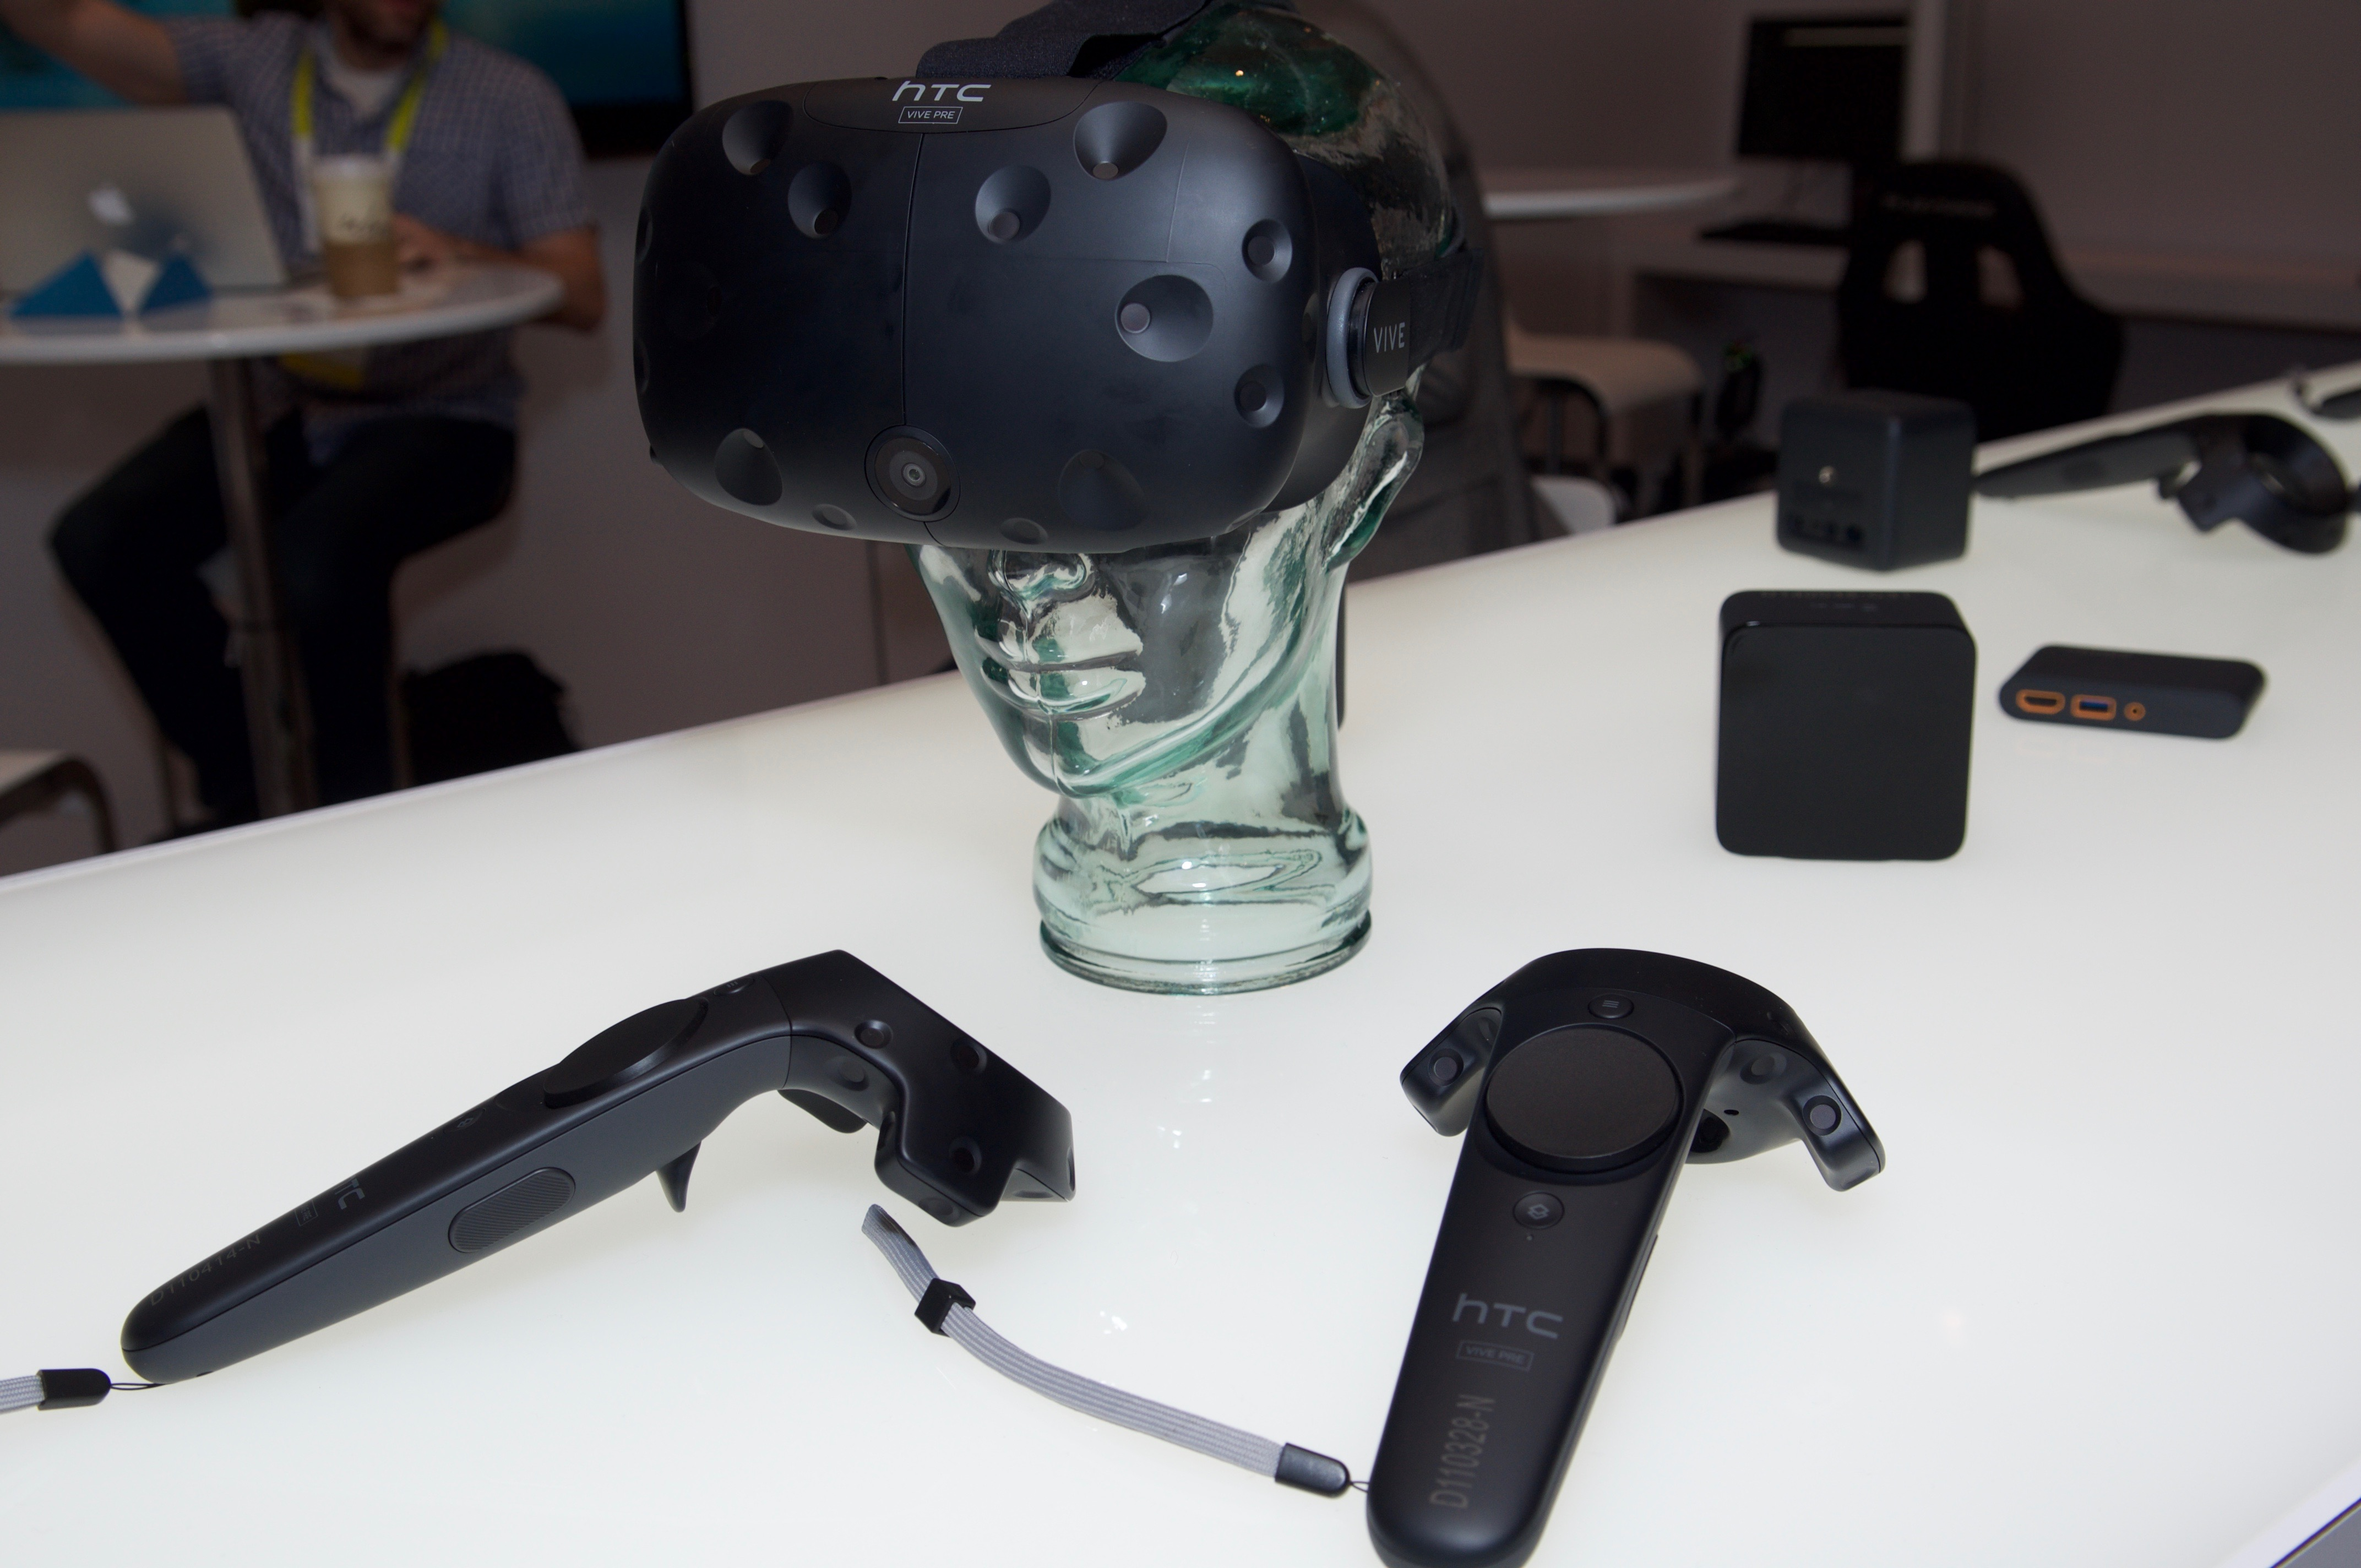
\includegraphics[width=12cm]{src/assets/vive-pre.jpeg}
\caption{Systém virtuální reality HTC Vive a jeho ovladače\autocite{htcvivepre}}
\end{figure}

\newpage

\section{Platforma Steam a SteamVR}\label{platforma-steam-a-steamvr}

Protože se na vývoji systému \emph{HTC Vive} podílela společnost
\emph{Valve}, je více než logické, že \emph{HTC Vive} je úzce spjat s
touto platformou.

Hry a aplikace určené pro tento systém jsou primárně distribuovány skrze
platformu \emph{Steam}. VR aplikace určené pro systém \emph{HTC Vive}
jsou pak podpořeny specializovanou platformou \emph{SteamVR}. Ta je
určena pro práci s hardwarem virtuální reality a jeho komunikaci s
počítačem. Je založena na open-source knihovně \emph{OpenVR}. V současné
době podporuje primárně jen systém \emph{HTC Vive} a v nedávné době byla
přidána experimentální podpora systémů \emph{Oculus Rift} a \emph{OSVR}. \autocite{steamvrsupports}

\emph{SteamVR} má na starosti spojení všech ovladačů a jejich
rozpoznání, a umožňuje systém z počítače ovládat (provést restart či
nastavení). V prostředí virtuální reality pak poskytuje možnost
konfigurace systému, zajišťuje, aby uživatel neopustil vyhrazený prostor
pro pohyb a další podpůrné funkce důležité pro nerušené zážitky ve
virtuální realitě.

\section{OpenVR}\label{openvr}

OpenVR je multi-platformní API rozhraní vyvíjené společností Steam,
které umožňuje snadný a rychlý přístup k hardware virtuální reality
různých výrobců. Poskytuje určitou míru abstrakce k tomu, aby vývojáři
měli přístup k jednotnému rozhraní bez závilosti na tom, jakého výrobce
systém právě používají.
